\uuid{MIpB}
\exo7id{7733}
\titre{exo7 7733}
\auteur{mourougane}
\organisation{exo7}
\datecreate{2021-08-11}
\isIndication{false}
\isCorrection{false}
\chapitre{Géométrie projective}
\sousChapitre{Géométrie projective}
\module{Algèbre et géométrie}
\niveau{L3}
\difficulte{}

\contenu{
\texte{
Soit $d$ et $d'$ deux droites d'un plan projectif.
Soit $h$ une homographie de $d$ dans $d'$ telle que $A'=h(A)$, $B'=h(B)$, $C'=h(C)$. Construire $h(M)$.

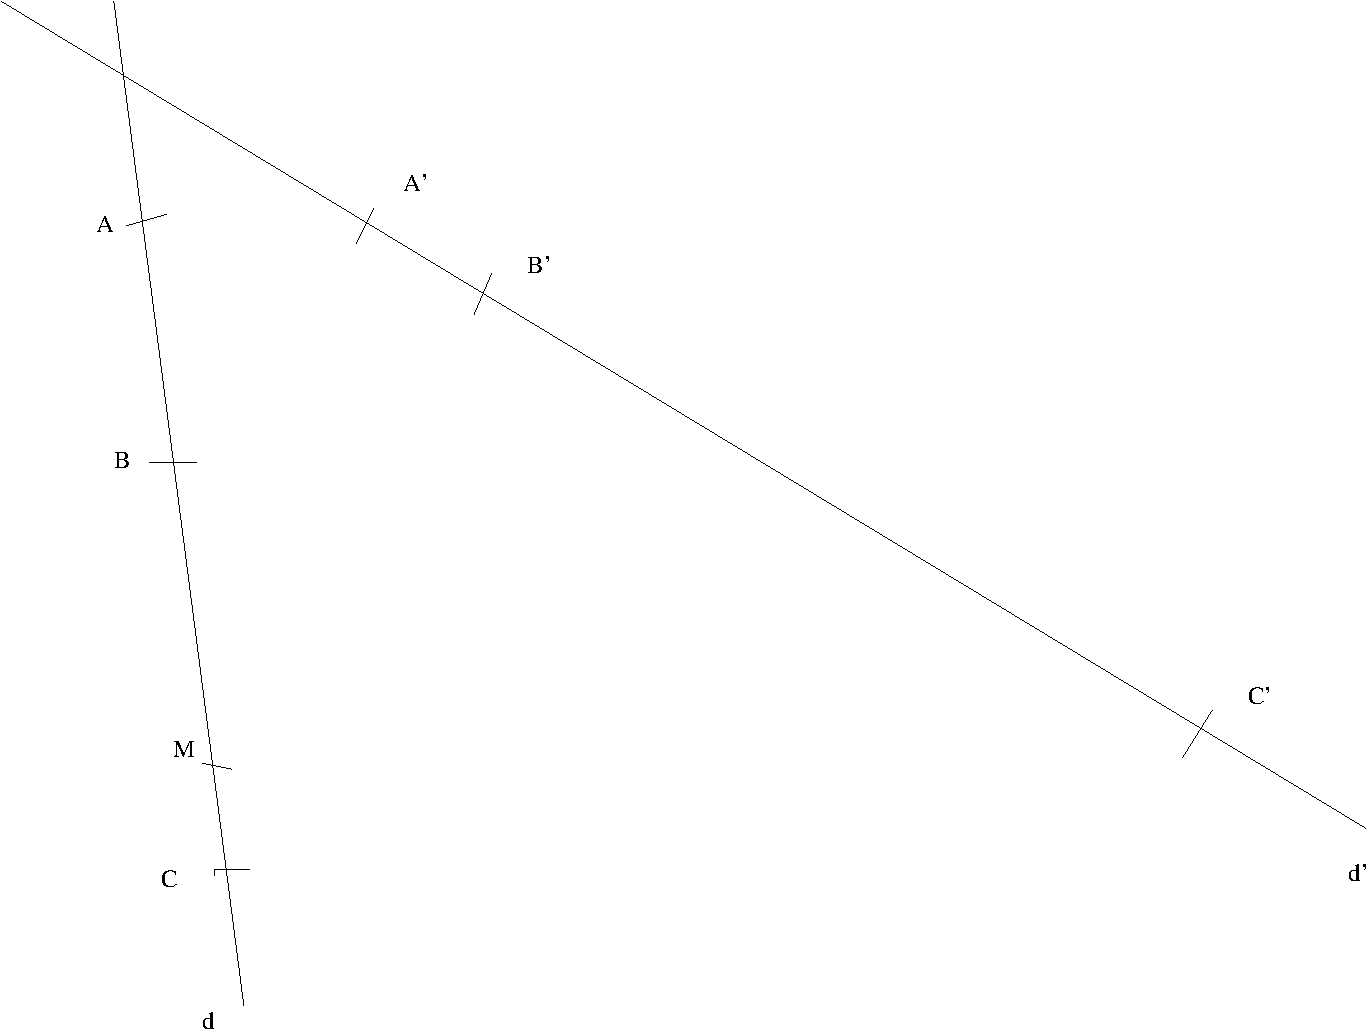
\includegraphics[scale=0.5]{images/pdf/MIpB-1.pdf}
}
}
